\documentclass{article}

\usepackage{amsmath}
\usepackage{graphicx}

\newcommand{\W}{{\mathcal W}}

\title{Numerical simulation of the shallow water circular hydraulic jump}

\author{
    David I. Ketcheson \and
    Manuel Quezada de Luna
}
\begin{document}

\maketitle

\begin{abstract}
We study numerical discretrizations of the shallow water equations
for the simulation of the circular hydraulic jump formed
when a vertical fluid jet impacts a horizontal plate.  
We focus on three numerical methods: finite volume Godunov-type
methods using either a Roe or HLLE approximate Riemann solver, and
a continuous Galerkin finite element method based on flux-corrected transport (FCT).
The finite volume methods are employed ona uniform cartesian grid
while the finite element method uses an unstructured triangular grid.
The three methods give completely different results, even for
highly-refined meshes.
\end{abstract}


\section{Introduction}

\subsection{The circular hydraulic jump}

Perhaps the first reference to the observation of the circular hydraulic jump
comes from Lord Rayleigh \cite{rayleigh1914theory}, who wrote that it
``may usually be seen whenever a stream of water from a tap strikes a horizontal
surface".  This phenomenon that is familiar in the everyday kitchen sink, is in
fact highly nonlinear and unintuitive.  Near the jet, the flow is very shallow and
fast, while further away it is deeper and slower.  The transition between these regions
occurs in a very narrow region and takes the form of \emph{jump} or \emph{bore}
that is roughly circular if the surface is flat; we refer to it herein as a
circular hydraulic jump (CHJ).

Early experimental work the CHJ began some time later
\cite{kurihara1946hydraulic,tani1949water,watson1964radial}.
Watson \cite{watson1964radial} worked out the jump radius
implied by Rayleigh's approach and then worked out the vertical
velocity profile in the inner region, assuming a no-slip
boundary condition at the bottom.  He also studied the turbulent
flow case and performed experiments.
More detailed experiments revealed different qualitative classification
of jumps  \cite{ishigai1977heat,craik1981circular}.
Although later work incorporated more physical details (such as surface tension) into the models
\cite{bush2003influence}, Bohr et. al. showed that important properties of the jump
(particularly its radius) could be reasonably predicted using a simple shallow water
model \cite{bohr1993shallow}.

While the jump is roughly circular, it may deviate from this shape and
deforming rapidly in time.
Instability of the jump was observed from fairly early on \cite{craik1981circular}.
Under special circumstances with more viscous fluids, the jump instability may lead to
the formation of curious shapes such as polygons \cite{ellegaard1998creating}, but
for a low-viscosity fluid like water the behavior is generally chaotic.
The instability increases with the jet velocity and with the depth at the outside of the jump,
and can be stable for sufficiently small velocities and depths.

\subsection{Numerical shock instabilities}

In \cite{peery1988blunt} a particular instability was observed to
appear in numerical simulation of a bow shock, near the symmetry plane.
This phenomenon, known as a ``carbuncle", has been observed by many researchers
in similar numerical experiments for the Euler equations, and many remedies
have been proposed, mainly in the form of additional numerical dissipation
\cite{quirk1997contribution,pandolfi2001numerical,dumbser2004matrix,chauvat2005shock,ismail2009proposed,shen2014stability}.
Most notably, the HLLE Riemann solver suppresses the carbuncle instability \cite{quirk1997contribution}.
For a recent review of numerical shock instability and work to alleviate it,
we refer to \cite[Section 2.5]{simonnumerical}.

Given the similarity of structure between the Euler equations and the shallow
water equations, one might expect carbuncles to appear in numerical
solutions of the latter as well.  Indeed, this has been observed \cite{kemm2014note}.
The shallow water carbuncle behaves in a fashion very similar to the
Euler carbuncle: it appears when the Roe solver is used, but not when
the HLL solver is used, and at least some of the other methods that suppress
the latter also suppress the former \cite{kemm2014note,bader2014carbuncle}.

Meanwhile, some research has suggested that the carbuncle is not purely a
numerical instability but instead is the manifestation of a true physical
instability \cite{moschetta2001carbuncle,elling2009carbuncle}.

\section{The shallow water circular hydraulic jump}
The shallow water equations in two (horizontal) dimensions are
\begin{align}
    h_t + (hu)_x + (hv)_y & = 0 \\
    (hu)_t + \left(hu^2 + \frac{1}{2}gh^2\right)_x + (huv)_y & = 0 \\
    (hv)_t + (huv)_x + \left(hv^2 + \frac{1}{2}gh^2\right)_y & = 0.
\end{align}
These can be written in vector form as
\begin{align}
    q_t + f(q)_x + g(q)_y & = 0.
\end{align}

\subsection{Semi-analytical solution under rotational symmetry}

\section{Numerical methods}

\subsection{Finite volume methods}

\subsubsection{Roe solver}

\subsubsection{HLLE (2-wave) solver}
The HLLE solver approximates the Riemann solution using two waves with
speeds $s_1, s_2$.  The middle state is
\begin{align} \label{qm-HLL}
    q_m^\textup{HLLE} = \frac{f(q_l) - f(q_r) + s_2 q_r - s_1 q_l}{s_2 - s_1}.
\end{align}


\subsubsection{A 3-wave solver}
Refinements of the HLLE solver were subsequently introduced in order to better
resolve contact and shear waves, which are strongly dissipated by the HLLE solver.
In the shallow water equations, we have only a shear wave.  We can introduce a third
wave in the approximate Riemann solver that carries the jump in the transverse velocity.
For simplicity, we describe this solver for an x-interface; i.e. where $u$ is the normal
velocity component and $v$ is the tangential velocity component.  Then the Riemann
solution is assumed to consist of 3 jump-discontinuities $\W^1, \W^*, \W^2$ where $\W^{1,2}$
carry all of the jump in $h$ and $hu$ while $\W^*$ carries all of the jump in $hv$.

The values $h_m$ and $u_m$, along with the speeds for the waves $\W^1,\W^2$ 
are thus determined by the same formula \eqref{qm-HLL} as in the HLL solver.
The speed of the middle wave is determined by conservation:
$$
    s^* = \frac{h_r v_r - h_l v_l}{h_r u_r v_r - h_l u_l v_l}.
$$
The middle state transverse velocity $v_*$ is given by $v_l$ if $s^*>0$ or $v_r$ if $s^*<0$.

\subsubsection{HLLEMCC solver}
The HLLEMCC approximate Riemann solver for the shallow water equations was proposed
in \cite{kemm2014note} specifically to deal with carbuncles.  The idea is to adjust
the amount of dissipation applied to the shear wave, adding dissipation in regions
where unphysical carbuncles would appear.  The approximate solution in this
case consists of four waves; the faster waves use the HLLE wave speeds and carry
jumps only in the depth and normal momentum, while the slower waves carry jumps
only in the transverse momentum.  By adjusting the value of $\phi$, this solver
can behave like the HLLE solver (if $\phi=1$) or like the Roe solver (if $\phi=0$).

The middle states $q^1_m, q^2_m$ are the same as those used for the HLLE solver.
Requiring conservation of the transverse momentum gives
$$
    q^3_m = \frac{f^3_l - f^3_r - (\hat{v}-\phi\hat{c})q^3_l + (\hat{v}+\phi\hat{c})q^3_r}{2\phi\hat{c}}.
$$
Here $\hat{v}, \hat{c}$ are the Roe-average normal velocity and sound speed, respectively.

\begin{figure}
    \center
    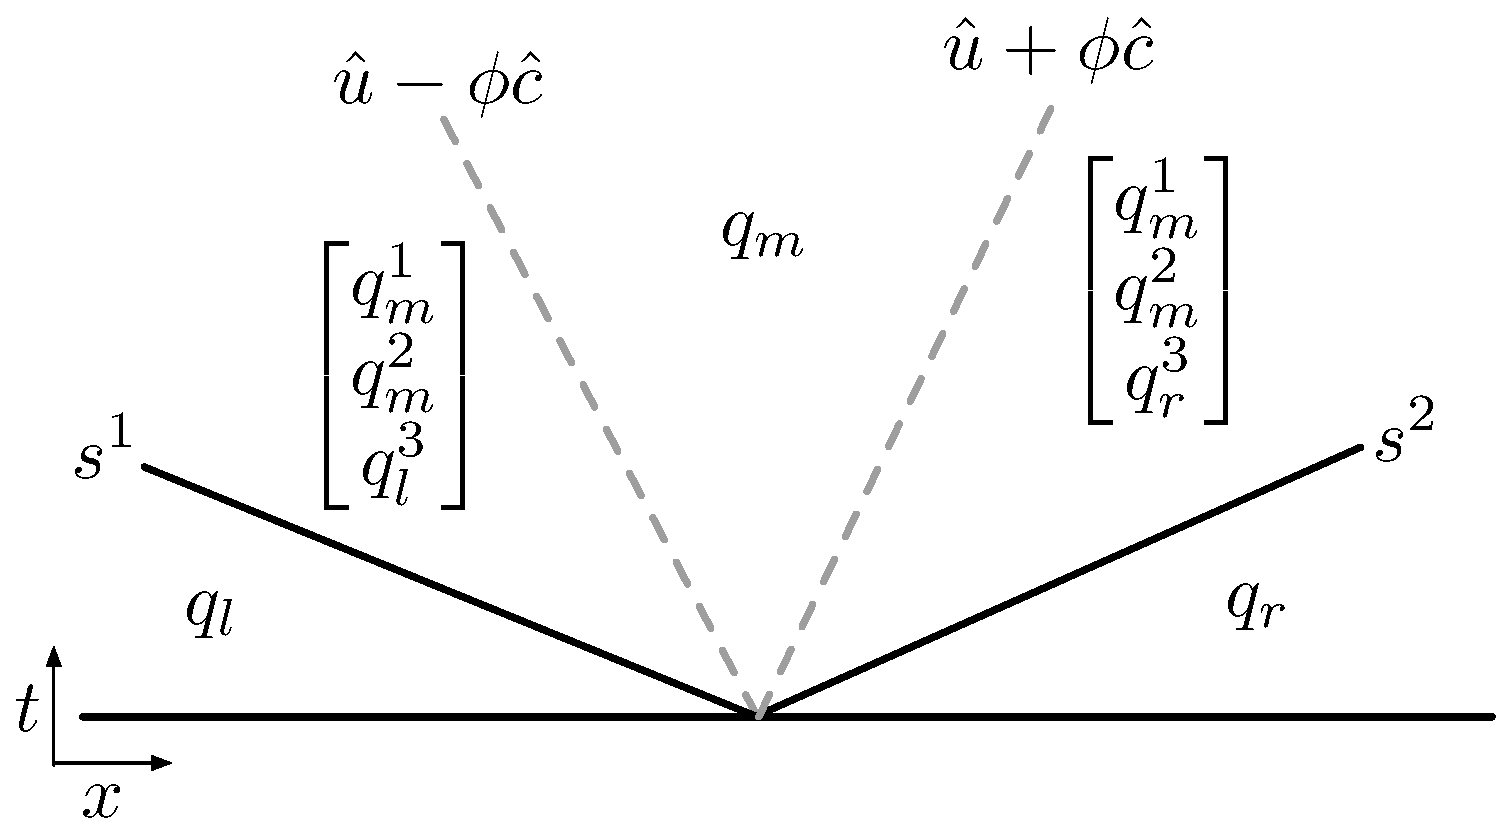
\includegraphics[width=0.6\textwidth]{figures/hllemcc.pdf}
    \caption{Structure of the HLLEMCC approximate Riemann solution, with four waves.}
\end{figure}

\subsection{Continuous Galerkin method}

\subsection{Discontinuous Galerkin method}

\section{Numerical results}

\subsection{Stable jump}

\subsection{Unstable jump}

\section{Conclusions}


\bibliographystyle{apalike}
\bibliography{refs}

\end{document}
